
% !TEX TS-program = pdflatex
% !TEX encoding = UTF-8 Unicode

%************************************************
\chapter{La Composizione}
\label{chp:La Composizione}
%************************************************

Delineati i tratti "somatici" di Sp.I.R.E. ho potuto finalmente immergermi nella stesura di una partitura \textit{ad hoc} per lo strumento. Tra i primi appunti:

\begin{itemize}
\item{il teatrale in musica. Ogni gesto ed ogni azione devono essere oltre che funzionali anche legata ad una spettacolarità.}
\item{Sp.I.R.E. è un nuovo mondo sonoro. Cercare di non subire esclusivamente la fascinazione dello strumento, ma lavorare anche su una struttura compositiva ben salda.}
\item{Interazione tra elettronica e microfoni tramite dei feedback indotti dal cambio di parametri (tramite i movimenti del pedale da parte del performer): filtri risonanti, modulazione di fase.}
\item{Costruire un elettronica misurata, che comprendesse, inoltre, la modulazione di frequenza e la modulazione ad anello, per l'amore che mi lega a questi processi di sintesi.}
\end{itemize}


\begin{wrapfigure}{r}{5cm}
\centering
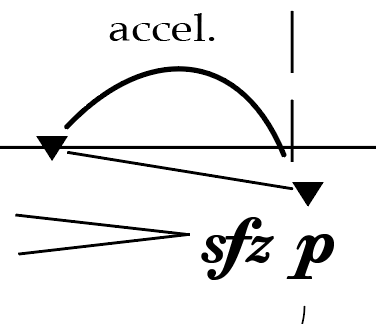
\includegraphics[width=.19\textwidth]{fig01.jpg}
\caption{particolare partitura \textit{Vitres de Son}}
\label{fig:part1}
\end{wrapfigure}

Ogni parte del brano è costruita su una quartina della poesia \textit{Vitres de Son}. Le righe della partitura si differenziano per piccoli tratti gestuali: ogni figura ha l'unione di uno o più timbri. In questo esempio, vediamo un pizzicato, dato dal simbolo triangolare\footnote{tutti i simboli verrano esplicati nella sezione dedicata alla legenda} e un glissato sulla molla, che produce uno strofinio (fig. \ref{part1}). 

L'insieme di più forme musicali sovrapposte per delineare un timbro complesso è una pratica cara al compositore \textit{Simone Santi Gubini}. Durante la sua masterclass \textit{Shock e ambiguità timbrica} tenutasi al Santa Cecilia durante \textit{EMUFest 2017} ci spiegò che l'utilizzo di più tecniche sovrapposte (fig. \ref{fig:gubini}) rende possibile un'assimilazione veloce del gesto e una chiarezza di linguaggio. 

\begin{figure}[htbp]
\begin{center}
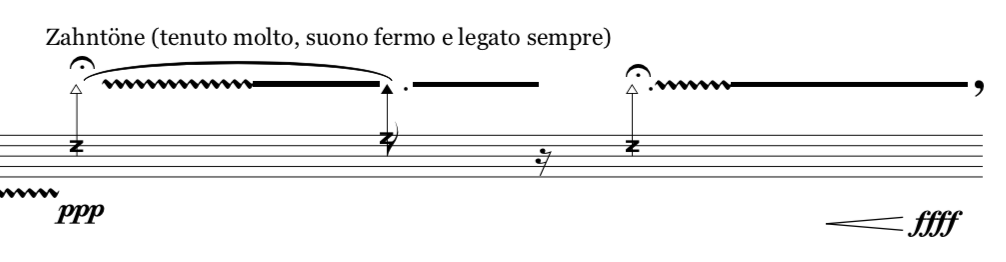
\includegraphics[width=.9\textwidth]{Gubini01.jpg}
\caption{Particolare partitura \textit{Klangrelief (Relief II)} di Simone Santi Gubini}
\label{fig:gubini}
\end{center}
\end{figure}

Così ho sfruttato tali insegnamenti per provare a sommare più simboli per arrivare ad un timbro complesso.
Tutte le figure ritmiche appaiono più come dei gesti musicali che come figure vere e proprie e fanno acquistare al pezzo delle caratteristiche prosodiche, come se ogni piccola cellula reciti un verso della poesia; per rendere possibile ciò, ho sillabato tutta la poesia, verso per verso, segnandomi le figure ritmiche (terzine, settimine) prodotte dagli accenti delle sillabe e i capoversi.

\section{Materiali sonori}

Vitres de son è stata composta, come detto, con un sistema che si può definire sia \textbf{Acustico} che \textbf{elettronico}\footnote{Acustica musicale e architettonica a cura di Sergio Cingolani, Renato Spagnolo UTET, 2004 Torino p. 3}.

%************************************************

\subsection*{I materiali acustici}

I rintocchi iniziali costruiti sulle molle danno vita a sub-armoniche e vanno ad enfatizzare le frequenze più gravi, mentre i suoni di sfondo formano dei continuum. Dal paesaggio sonoro, dal soundscape fatto di piccoli grattati in \textbf{\textit{ppp}}, emergono le sillabe dei versi, come se prendessero forma piccoli respiri dati dalla lettura delle parole del poeta. Appare un \textit{dramma}, un enorme piaga che sottolinea Artaud in tutta la sua poetica giovanile e nei suoi lavori teatrali: non c'è più linguaggio parlato, divincolato dalla struttura principale di diffusione orale, ma solo suono.

%************************************************

\subsection*{L'elettronica}

Le varie parti di modulazione di frequenza e le interazioni ritmiche si incastrano seguendo un movimento verso le frequenze più alte. la notazione si erige, come grande rosone, verso armoniche generate sia dal materiale metallico, sia dai contributi dell'elettronica.  Si va ad indagare \textit{nello} strumento (tramite una scrittura prettamente legata all'universo delle percussioni) sia \textit{sullo} strumento (tramite l'utilizzo dell'elettronica). Ogni contributo elettronico è un valore \textit{intrinseco} a Sp.I.R.E. che lascia riecheggiare nell'ambiente circostante tutte le sue risonanze.

%************************************************

\section{Idea ritmico-melodica}

Ho cercato di creare una cellula di suoni disposti orizzontalmente, per poi lavorare sulla parte contrappuntistica. Dato che il nuovo strumento non ha \textit{pitch} definiti è stato complicato lavorare su una cellula che al finire del suo svolgersi si potesse considerare conclusa. Ho provato ad utilizzare degli stratagemmi musicali, come accenti o determinati effetti timbrici (ad esempio attivazione di armoniche sugli estremi delle molle) su ogni figura ritmica. Queste cellule ritmico-melodiche sono l'interazione con la materia di cui è composto lo strumento, sempre con un rapporto di 1:1 tra il ferro armonico delle placche e il metallo armoniche delle molle.
Sarà poi l'elettronica e i continuum a legare tali figure ritmiche. Si noti, durante la performance, che alcune scelte gestuali presenti in partitura, sono connesse ad un movimento esclusivamente performativo: quasi teatrale (ad es. l'incrocio degli archetti nella III parte sulle placche 2 e 3).

Le figure ritmiche servono a dare alla composizione un andamento strutturale. Ovvero, le figure sono legate ad un preciso \textit{ictus}, servono a creare degli incontri come ad esempio quelli tra elettronica e parte strumentale o nell'incastro verticale delle voci. Nelle figure ritmiche di \textit{Vitres de Son}  (fig. \ref{fig:sill}) sono nascoste le sillabazioni dei versi (andamento "vocale" delle parti).


\begin{figure}[htbp]
\begin{center}
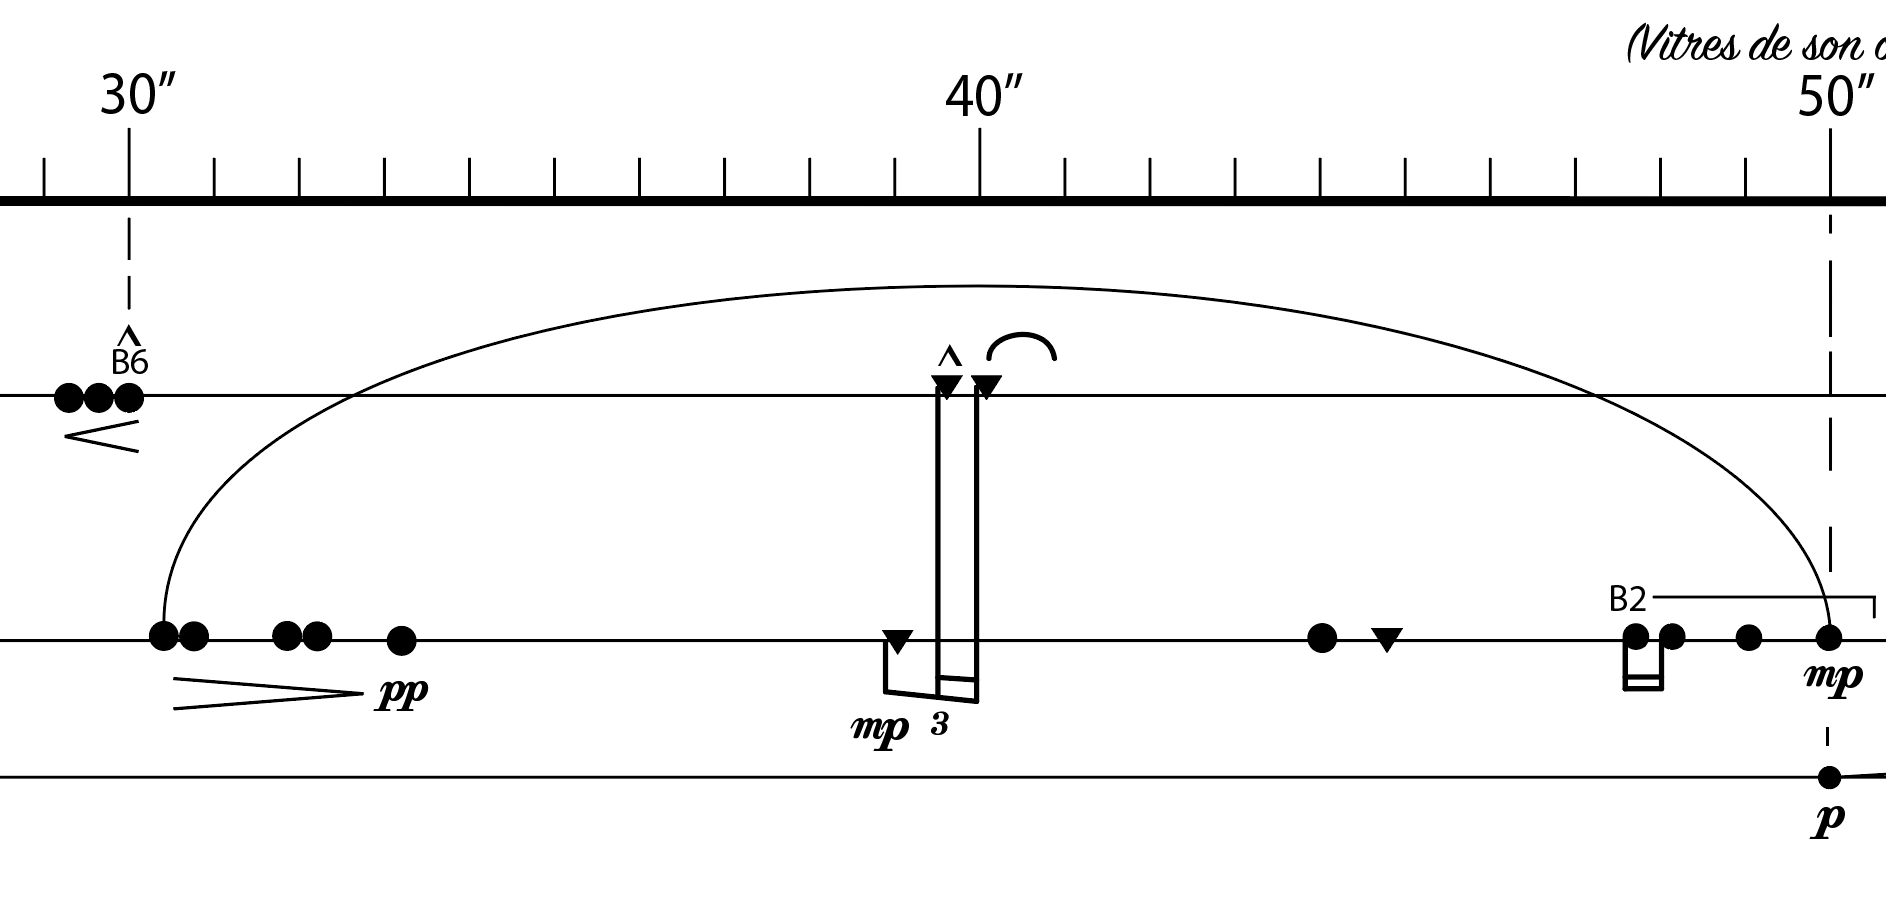
\includegraphics[width=.99\textwidth]{sillabaritmica.jpg}
\caption{\textit{Esempio di sillaba ritmica}}
\label{fig:sill}
\end{center}
\end{figure}

Ho considerato utili tecniche di scrittura contemporanea legate al mondo degli idiofoni e all'universo dei cordofoni.

Per quanto riguarda la notazione, ho trovato, nel libro sulla semiografia contemporanea di Luigi Donora\footnote{Luigi Donora, \textit{Semiografia della nuova musica}, }, molte delucidazioni sulla creazione di figure ritmiche e simboli che potessero al meglio rappresentare il mio fine compositivo. Per fine compositivo intendo la possibilità di creare determinati timbri, riportando notazioni non canoniche ma che facessero capire la tipologia di gesto da utilizzare in un determinato frammento. Durante la stesura della partitura ha cambiato forma diverse volte. La prima partitura, infatti, era stata creata direttamente su una serie di pentagrammi, dove il SI sopra al DO centrale  simboleggiava il centro della molla e il movimento verso il basso o verso l'alto delle note rappresentava rispettivamente un movimento verso sinistra o verso destra.

%************************************************

\section{Gestualità}

La fortuna di questo strumento è che per metà è acustico e che la sua curva di decadimento è molto larga. La puntualità in partitura nel far capire quali punti della molla colpire è alla base di un gesto preciso, che possa essere sempre lo stesso per lo stesso simbolo scritto e per la stessa risultante sonora. La legenda, quindi, oltre ad avere l'esplicazione della simbologia, ha anche dei piccoli esempi di qualche rigo della partitura o dell'utilizzo del pedale; in alcuni casi può risultare estremamente efficace per migliorare l'esecuzione del brano. Il pretesto di utilizzare i versi di una poesia può essere in parte affiliata ad una sostituzione della parola con il gesto che produce il suono. 

\begin{figure}[htbp]
\begin{center}
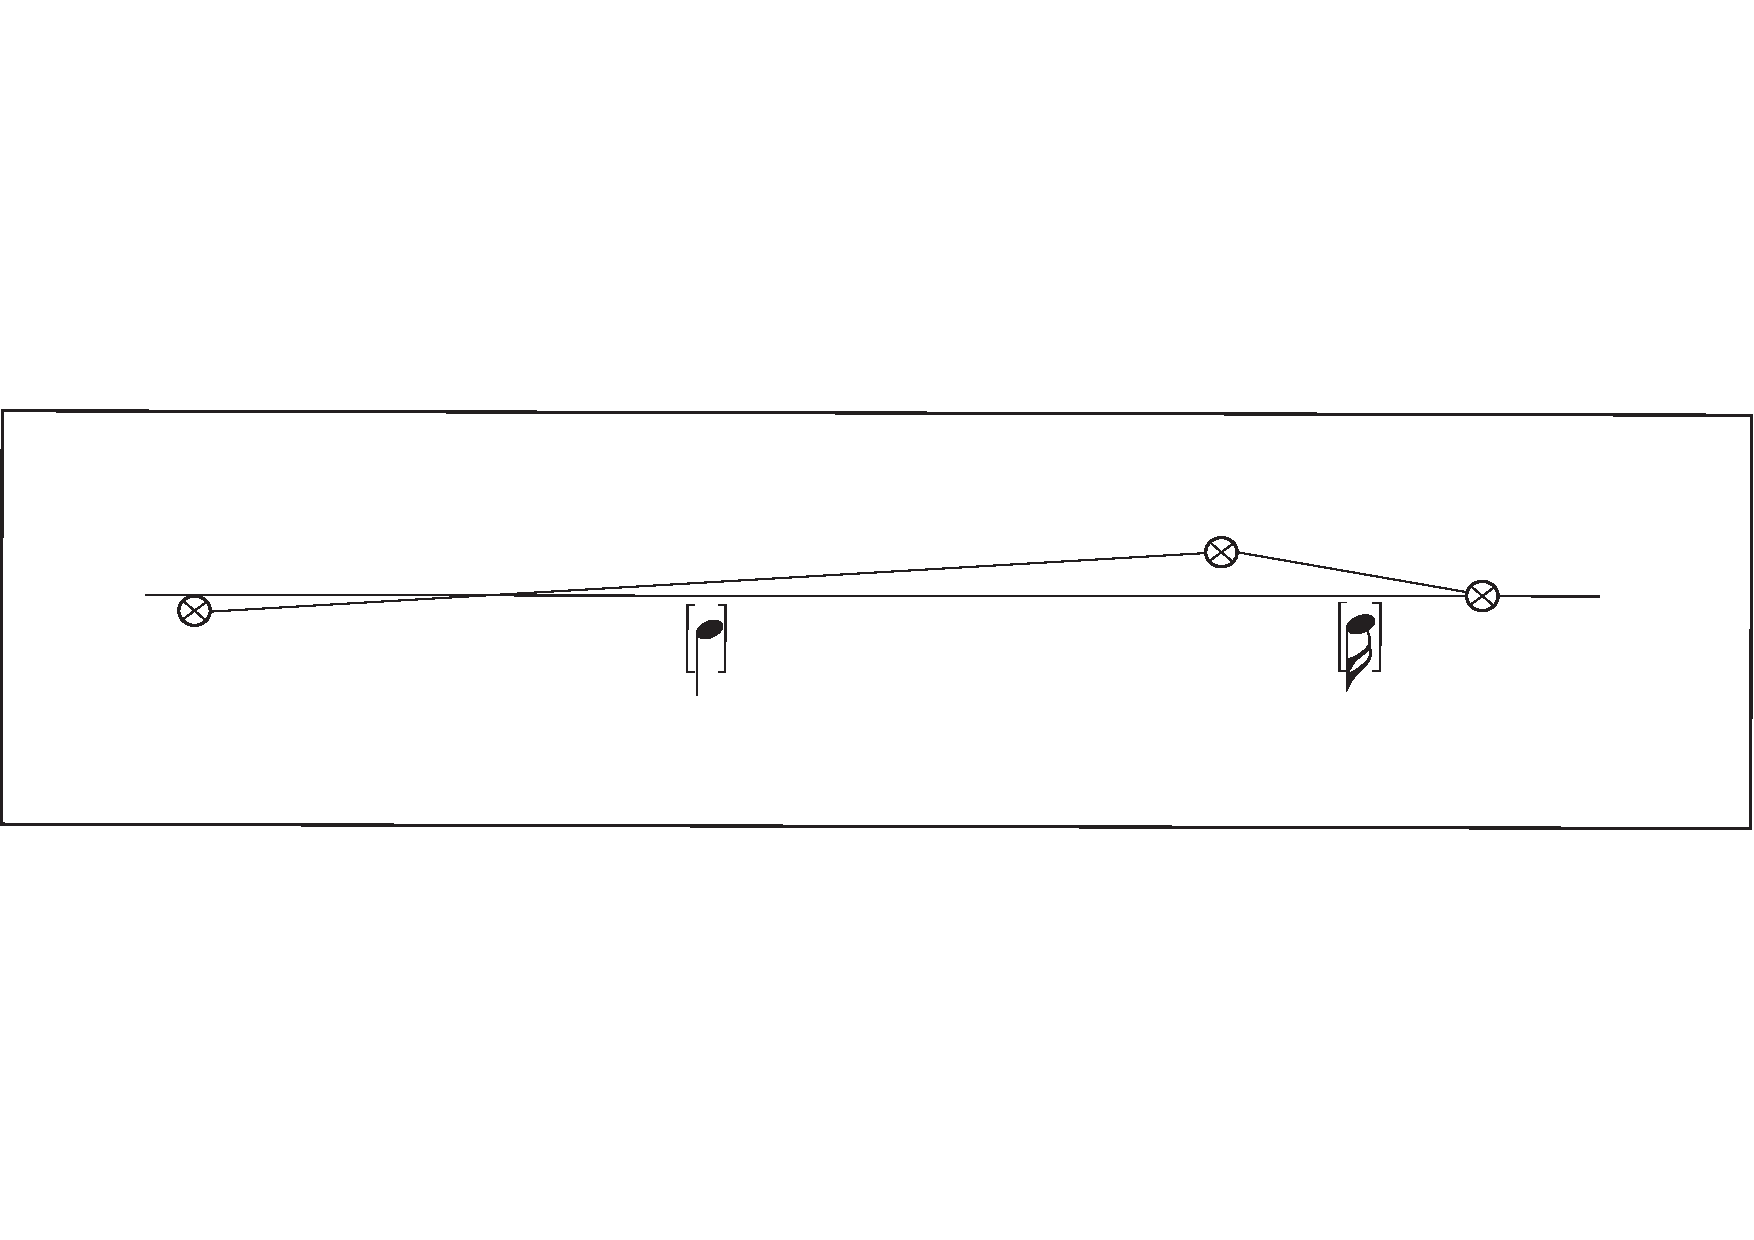
\includegraphics[width=0.99\textwidth]{Legenda4.pdf}
\caption{\textit{Particolare \textit{Vitres de Son}}}
\label{fig:vitres}
\end{center}
\end{figure}

Continuando l'analisi della partitura, notiamo che ha, come oggetto principale di scrittura, il processo con il quale sono stati ricercati i suoni: ogni simbolo grafico rappresenta un gesto (fig. \ref{fig:vitres}). Non viene perciò rappresentata la risultante timbrica, ma piuttosto il processo con il quale si va a produrre un determinato suono. Sarà, quindi, il gesto ad essere la base della prosodia interna, ogni legame con il gesto successivo sarà studiato per dare sia un movimento alle voci, che possono essere sino a 3 simultanee (come si nota nel solo sulla molla 5), sia per dare una sensazione di continuum.

L'utilizzo di simboli vicini al mondo della musica classica mi ha aiutato ad adeguare uno strumento del quale non abbiamo letteratura verso una nuova scrittura. Questo procedimento è la base poi della musica contemporanea, ovvero, ogni nuovo gesto è la decodifica di un simbolo evoluzione di musica più antica.

Alcuni movimenti scritti per l'archetto, infatti, stanno a simboleggiare un gesto, come avveniva in passato per la musica gregoriana, con i \text{melismi} legati al movimento delle mani del direttore di canto gregoriano.

%\begin{figure}[htbp]
%\begin{center}
%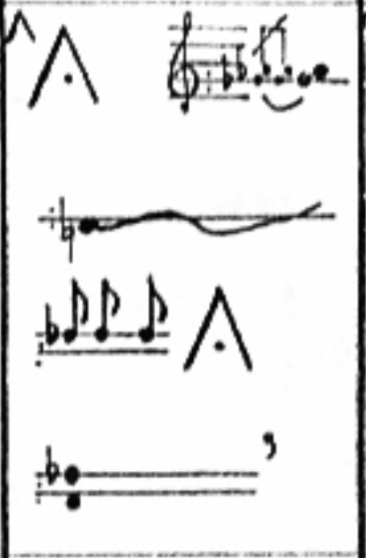
\includegraphics[width=0.19\textwidth]{guaccero01.jpg}
%\caption{\textit{Particolare di Sinfonia 1 di Domenico Guaccero}}
%\label{default}
%\end{center}
%\end{figure}

\clearpage

\thispagestyle{empty}

\includepdf[offset=-30 10,
		    scale=1.,
		    pagecommand={
		    	\begin{tikzpicture}[
					remember picture,
					overlay]
		    	\node [xshift=10cm,yshift=1cm] at (current page.south west) {\color{white}{}};
				\end{tikzpicture}}
		    ]{Macroforma01.pdf}

\clearpage
Analizzando brevemente la partitura, si nota che, come oggetto principale della scrittura c'è il processo con il quale i suoni sono stati ricercati: ogni simbolo grafico rappresenta un gesto. Nono viene perciò rappresentata in molti casi la risultante timbrica, ma piuttosto il processo con il quale si va a produrre un determinato suono. Sarà, quindi, necessario che il gesto sia la base di una prosodia interna e che ci sia un legame con il gesto successivo. In alcuni punti (soprattutto nell'utilizzo degli archetti o per la formazione del continuum o per i movimenti del pedeale) ci sono delle linee che disegnano appunto il gesto che il performer dovrà fare. Ogni linea è come una sorta di \text{melisma} in contrapposizione al movimento \textit{sillabico}. Potrei accostare addirittura la partitura di Vitres de Son, ai lavori di Domenico Guaccero, come ad esempio \textit{Sinfonia I}, dove oltre ad una notazione standard aggiunge delle linee legate ad un gesto musicale.

\begin{figure}[htbp]
\begin{center}
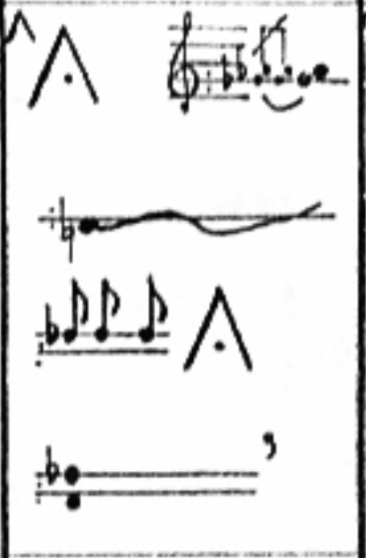
\includegraphics[width=0.19\textwidth]{guaccero01.jpg}
\caption{\textit{Particolare di Sinfonia 1 di Domenico Guaccero}}
\label{fig:guacc02}
\end{center}
\end{figure}

%************************************************%************************************************%************************************************%************************************************

\section{Macro-forma}

%************************************************

La struttura complessiva del brano è tripartita. 

Nella pagina precedente, la rappresentazione grafica della Macro-forma di Vitres de Son. Di seguito, la spiegazione delle tre parti che compongono il brano.

\subsection*{I Parte}

L'incipit è dato da una forma distesa piena di frequenze basse che somigliano a dei rintocchi. Qui iniziano a prendere vita le prime cellule ritmiche, cercando di andare di pari passo con una lettura temporale della poesia di Artaud: dalla vista dal basso verso l'alto degli astri (\textit{verres où cuisent les cerveaux / le ciel fourmillant d'impudeurs}).

%************************************************

\subsection*{II Parte}

Ho congiunto le varie forme ritmiche con delle parti di soundscape costruito grazie a un tremolo lento sulle molle più grandi. Tali macchie di suono rendono possibile lo sviluppo di un continuum che si manifesta in lontananza per riaffiorare in alcuni punti, decadendo velocemente, seguito da vertiginose corse delle dita sulle molle. Ogni cellula che si va a formare, si ripete, ma con piccole variazione, con code differenti. Ogni gesto è riconosciuto sia nella semiografia che dal timbro percepito. L'elettronica entra in sordina, si adagia nel sottosuolo dei pianissimo ed emerge a tratti (in contrappunto con i tremoli) sempre più delineati, fino a sfociare in un feedback controllato sul solo della Molla 5. 

%************************************************

\subsection*{III Parte}

Un piccolo intermezzo divide la parte II dalla III, uno spartiacque tra un continuum  e il successivo. Il secondo continuum non è un passaggio di personaggi sonori (le molle), ma è l'evoluzione dei gesti sulle lastre, che da leggera patina sonora si trasformano in stridenti movimenti d'archetto che convogliano in una serie di jeté (\textit{un tourbillon d'ailes sauvages}) per sfociare definitivamente in arcate pesanti su lastre opposte fino al crescendo finale. La struttura della III parte è tutta una preparazione a questo crescendo che culmina nei decadimenti acustici di Sp.I.R.E..

%************************************************

Nello stesso modo con il quale si applicano modifiche a livello di velocità di emissione delle sillabe durante una recitazione, così ho cercato di dar vita a delle variazioni nelle strutture ritmiche che si fondo con l'universo sonoro sottostante e vengono inghiottite dal soundscape. Ciò è reso possibile dalla natura del materiale: ogni passaggio delle dita o unghie sulle spire delle molle crea dei micro-glissati che formano maglie di suono che si fondono con le elaborazioni del live electronics. Ad un tratto appare, su frequenze gravi, una modulazione di frequenza. Questa FM, al suo interno ha dei piccoli movimenti spettrali, legati ad altrettanto piccole variazioni di parametri interni. Come affermava Xenakis:

\begin{quotation}
Una moltitudine di brevi \textit{glissandi} può dare l'impressione del continuo, come anche una moltitudine di \textit{pizzicati}\footnote{Iannis Xenakis, \textit{Universi del suono, Scritti e interventi 1955-1994} (a cura di Agostino Di Scipio), Ricordi S.r.l. e LIM Editrice S.r.l., 2003}.
\end{quotation}

\section{La legenda}
La partitura si apre con la macroforma, l'amplificazione e il sistema algoritmico, per poterlo riprodurre con i giusti materiali sonori.\\
Per facilitare la lettura della partitura elettroacustica, ho preferito dividere la legenda in quattro blocchi fondamentali:
\begin{itemize}
\item{Il primo blocco comprende la tipologia di battenti, utilizzati anche nella musica classica, ma \textit{numerati}, per facilitare i cambi in partitura, dato che per ogni battente, abbiamo un'eccitazione diversa delle molle e, quindi, un timbro differente.}
\item{Il secondo blocco delinea la notazione e la simbologia.}
\item{Il terzo blocco ha degli esempi, che facilitano lo studio degli incastri ritmici}
\item{L'ultimo blocco comprende tutti i simboli e i gesti legati all'elettronica (pedali, variazioni di parametri, elaborazioni)}
\end{itemize}

\clearpage

\thispagestyle{empty}

\includepdf[offset=0 0,
		    scale=0.9,
		    pagecommand={
		    	\begin{tikzpicture}[
					remember picture,
					overlay]
		    	\node [xshift=10cm,yshift=1cm] at (current page.south west) {\color{white}{}};
				\end{tikzpicture}}
		    ]{legenda2.pdf}

\clearpage

\clearpage

\thispagestyle{empty}

\includepdf[offset=-10 0,
		    scale=1.,
		    pagecommand={
		    	\begin{tikzpicture}[
					remember picture,
					overlay]
		    	\node [xshift=10cm,yshift=1cm] at (current page.south west) {\color{white}{}};
				\end{tikzpicture}}
		    ]{legenda3.pdf}

\clearpage

\section{Algoritmi}

Tutti gli algoritmi sono stati disegnati prendendo ad esempio la simbologia esplicata da Walter Branchi nell'appendice 6 del libro \textit{Tecnologia della musica elettronica}\footnote{Walter Branchi, \textit{Tecnologia della musica elettronica} (con prefazione di Domenico Guaccero), Lerici, Roma, 1977}. Lo schema completo presente in partitura è vicino ad una visione sia di riproducibilità, che di visione globale, nella quale si intravede, già nello schema algoritmico il pensiero compositivo che c'è sotto (un altro schema algoritmico che ho preso da esempio è stato \textit{Audible Ecosystemics 2} di Agostino di Scipio).

Tecniche di sintesi utilizzate:

\begin{itemize}
\item{Sintesi Granulare, 8 voci}
\item{Modulazione di frequenza, 12 voci}
\item{Modulazione di ampiezza}
\item{Modulazione ad anello}
\item{Filtro Risonante}
\end{itemize}

\clearpage

\thispagestyle{empty}

\includepdf[offset=5 0,
		    scale=.90,
		    pagecommand={
		    	\begin{tikzpicture}[
					remember picture,
					overlay]
		    	\node [xshift=10cm,yshift=1cm] at (current page.south west) {\color{white}{}};
				\end{tikzpicture}}
		    ]{Algoritmica.pdf}

\clearpage

\section{Pedaliera}

Dopo aver studiato il funzionamento della pedaliera, ho notato che ogni pulsante numerato era assegnato ad un NOTE on, come una normalissima pedaliera midi per organo. La fortuna è che ogni pulsante equivale a note inerenti al numero presente sulla pedaliera (es. note-on 1 = tasto 1 pedaliera). Quindi essendo identiche, ho solo dovuto trasformare ogni note-on in un "lancio-scena" sul mio software di utilizzo (max-msp). Questo mi ha facilitato lo studio con il performer che poteva riprovare ogni scena senza doverle ripetere in sequenza temporale: ovvero poteva passare dalla scena 1 alla scena 6 senza dover ripercorrere tutte le scene presenti tra quelle menzionate. Questo ha facilitato di gran lunga le prove fatte per ogni singolo rigo.
